\documentclass[10pt, conference, letterpaper]{IEEEtran}
\usepackage{cite}
\usepackage{xcolor,soul,framed}
\usepackage{amsmath,amsthm,amssymb,amsfonts}
\usepackage{algorithmic}
\usepackage{graphicx}
\usepackage{color, soul}
\usepackage{algorithm, algorithmic}
\usepackage[utf8]{inputenc}
\usepackage[english]{babel}
\usepackage{mathtools}
\graphicspath{ {./images/} }

%---------------------------------------------------------------%
\newtheorem{definition}{Denifition}
\newtheorem{assumption}{Assumption}
\newtheorem{problem}{Problem}
\newtheorem{lemma}{Lemma}
\newtheorem{corollary}{Corollary}
\newtheorem{example}{Example}
\newcommand{\eq}{=}
\newcommand{\domZ}{\mathbb{Z}_{*}}
\newcommand{\vecOne}{\mathbf{1}}
\newcommand{\ind}{\mathbf{I}}
\newcommand{\mat}{\mathbf}
\newcommand{\define}{\triangleq}
\newcommand{\leadto}{\Rightarrow}
\renewcommand{\vec}{\mathbf}
\DeclarePairedDelimiter{\set}{\{}{\}}
\DeclarePairedDelimiter{\norm}{|}{|}
\DeclarePairedDelimiter{\Inorm}{\|}{\|_1}
% \DeclarePairedDelimiter{\set}{\bigg(}{\bigg)}
%---------------------------------------------------------------%
\newcommand{\apSet}{\mathcal{K}}
\newcommand{\esSet}{\mathcal{M}}
\newcommand{\jSpace}{\mathcal{J}}
\newcommand{\wSet}{\mathcal{W}}
\newcommand{\uSet}{\mathcal{U}}
\newcommand{\cSet}{\mathcal{C}}
\newcommand{\Stat}{\mathbf{S}}
\newcommand{\Obsv}{\mathcal{X}}
\newcommand{\Policy}{\mathbf{\Omega}}
%---------------------------------------------------------------%

\begin{document}

    %=============================== TITLE ===============================%
    \title{
        Meet-in-Future: Distributed Online Job Dispatching with Obsolete Information in Edge Computing System
    }
    \author{
        \IEEEauthorblockN{Yuncong Hong$^{*\dagger}$}
        \IEEEauthorblockA{
            $*$Southern University of Science and Technology, P.R. China,
            $\dagger$The University of Hong Kong, Hong Kong,\\
            $\ddagger$University of Science and Technology of China, P.R. China
        }
    }
    \maketitle

    %============================== ABSTRACT ==============================%
    \begin{abstract}
        \label{sec:abstract}
        Edge computing is believed to be the solid solution for time-sensitive big data real-time calculation. The cooperation among edge servers in the same coalition usually causes ineffective task scheduling due to obsolete information sharing, which is hard to tackle even with extra centralized agent design. In this work, we formulate the problem with job dispatching in distributed Edge Computing system, and identify the difficulty exists in cooperation between AP nodes (Access Points) and ES nodes (Edge Servers) with delayed information. We design the broadcast information in the system and formulate the corresponding problem into a MDP problem. The value function approximation and \st{one-step policy iteration method is adopted to obtain a sub-optimal dispatching policy whose performance can be bounded analytically}.
    \end{abstract}

    % \begin{IEEEkeywords}
    %     Edge Computing, Job Dispatch, Delayed Information, Collective Observability, Distributed Multi-agent MDP
    % \end{IEEEkeywords}

    %============================ INTRODUCTION ============================%
    \begin{section}{INTRODUCTION}
        \label{sec:introduction}
        Our claims:
        \begin{itemize}
            \item Related works on job dispatching on scheduling in edge computing, mostly with centralized agent to apply action and seldomly take delayed information impact into consideration;
            \item Edge Server, Access Point, User Equipment; layered structure where decision is made distributedly on AP nodes and computation is carried out on ESs; The AP-ES fully separated structure is reasonable, for example C-RAN to separate communication and computation resource assembling;
            \item We identify the delayed system information is un-acceptable for explosion \emph{delay-sensitive jobs} in edge computing, and it's hard to establish cooperation among AP nodes because of obsolete information;
            \item information sharing for cooperation is designed via (aligned) broadcast, job dispatch decision should be made immediately based on the previous collective information;
        \end{itemize}

        Our contributions:
        \begin{itemize}
            \item identify that the uploading process affect the performance of heuristic greedy algorithm; identify that the delay-information sharing in decision making;
            \item propose a instantaneous job dispatching scheme in a fully-distributed cooperative way;
            \item propose global consensus state method to formulate the multi-agent MDP problem;
            \item adopt value function approximation to reduce the traditional algorithm complexity, and come up with distributed online learning algorithm;
        \end{itemize}

        Related works:
        \begin{itemize}
            \item The earliest related works we find is \cite{ref-01} (cited 167 times). In this work, the single agent is assumed not able to observe the global state, and thus they need communication to establish cooperation by sharing \emph{information}. The agent considers communication as extra action to synchronize the states and thus incurs extra cost. \\
            However, the communication is without delay, and converted into POMDP problem.
            \item The other work \cite{ref-02} considers continuous state observation with constant or stochastic delay with single agent.
        \end{itemize}

        Bulky Reference List for Journals:
        \begin{itemize}
            \item \text{[IoT,out-of-date]} \cite{Lyu2017} is work considering \emph{out-of-date knowledge} optimization in IoT computing scenario;
            \item
                \cite{Yang2016} is a work considering services placement and requests dispatching on edge servers, and leverage users' pattern to predict "service cache" for online decision making;
                \cite{Du2018} is a work considering computation offloading and computation resource allocation to satisfy min-max fairness guarantee, under minimum tolerant delay;
                \\
                \cite{Chen2016} is a work considering multi-user computation offloading with multi-channel contention, and adopt game theory approach to achieve Nash equilibrium with upper bound of convergence time;
                \cite{Rodrigues2017} is a work on minimizing service delay in mobile edge computing;
                \cite{Wang2017} is a work considering service placement with graph theory;
            \item \text{[foggy]}
                \cite{Masip-Bruin2016} is a work with layered structure with foggy and cloud computation;
            \item \text{[unfinished]}
                \cite{Fan2017}; \cite{Lyu2018}; \cite{Lyu2018a}; \cite{Chen2018}; \cite{Yu2018}; \cite{Zhang2018}; \cite{Wang2018}; \cite{Josilo2019}; \cite{Chen2018a}; \cite{Sthapit2018}; \cite{Naha2018}; \cite{Dinh2018}; \cite{Lyu2018b}; \cite{Garcia-Saavedra2018};
        \end{itemize}

    \end{section}

    %============================ SYSTEM MODEL ============================%
    \begin{section}{SYSTEM MODEL}
        \label{sec:model}
        \begin{subsection}{Network Model}
            The network topology of the MEC (mobile edge computing) system in this article is composed of three components as illustrated in Fig. \ref{fig:system}.
            The user equipment (UE) is connected to access point (AP) and offloads computation jobs to access point. The AP itself is assumed with no computation capability, and thus it need to further dispatch those jobs to the edge servers (ES) in the same coalition. There are more than one AP nodes in the MEC system, which determines that the ES should complete the jobs computation \textcolor{red}{in a fairness way}. The network topology between AP cluster and ES cluster is fully accessible so that AP could dispatch jobs to any ES nodes in this coalition.

            In this MEC system, we adopt the same timing mechanism at both AP and ES side with a minimum \emph{timeslot} lasting for $\kappa$ seconds, which is indexed with symbol $t$. The timing precision among all the nodes is promised with a timing protocol (e.g. GPS Timing) and is beyond the discussion of this article. The dispatching and scheduling decision on AP and ES side respectively are all applied based on this timing. Moreover, the information sharing in this coalition is designed via broadcast design which will be elaborated in \emph{Information-Sharing Broadcast Model} section.

            Now we give the formal definition of the network illustration. Let $\apSet \define \set{1,\dots,K}$ and $\mathcal{M} \define \set{1,\dots,M}$ denote the set of AP nodes and set of ES nodes in the MEC system respectively. The computation jobs offloaded from UEs connected with $k$-th AP ($\forall k\in\apSet$) is denoted as \emph{job arrival process} which follows the assumption as:
            \begin{assumption}
                (Job Arrival Process at $k$-th AP).
                We denote the job arrival process for $k$-th AP as $A_k(t)$ which is i.i.d over each timeslot with Bernoulli distribution $A_k(t) \sim Bernoulli(\lambda_k)$. The Bernoulli distribution implies that there will be at most one job arrives on $k$-thAP in one timeslot. According to Poisson Limit Theorem, we identify that the arrival process is a memory-less exponential process with average arrival rate $\mathbb{E}[A_k(t)] = \lambda_k$.
            \end{assumption}
            
            \begin{figure}[ht]
                \centering
                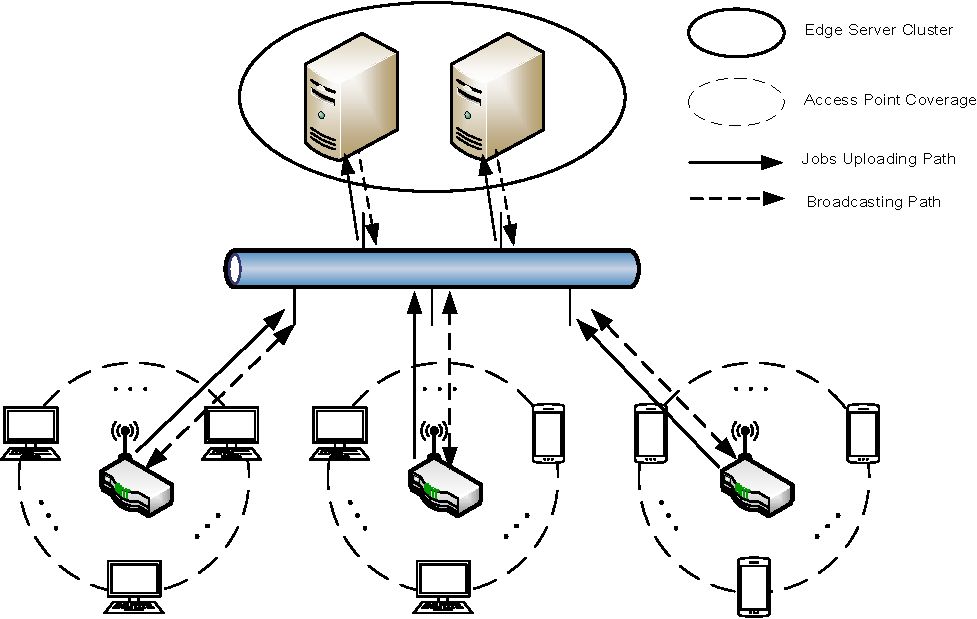
\includegraphics[width=0.45\textwidth, trim={0.5cm 0.5cm 0.5cm 0.5cm}, clip]{system-model.pdf}
                \caption{The Illustration of MEC System Model}
                \label{fig:system}
            \end{figure}

            The offloaded jobs in each timeslot are then immediately dispatched to edge servers which compose the \emph{uploading process} over all AP-ES paired links. We assume that the uploading delay is independent of computation job types and is deterministic for one AP-ES link, which is denoted as $t^{u}_{k,m}$ timeslots from $k$-th AP to $m$-th ES ($\forall k\in\apSet, \forall m\in\esSet$).
            The \emph{parallel uploading} is enabled on AP nodes to alleviate the extra waiting cost caused by serially uploading. As the arrival process and uploading time is bounded, there will be at most $\lambda_k \cdot \max_m(t^{(u)}_{k,m})$ jobs in transmission on $k$-th AP which results into finite bandwidth allocation.
        \end{subsection}

        \begin{subsection}{Computation Model}
            For computation process on edge servers, we adopt \emph{unrelated machines} assumption in \cite{tan-online}, where the job processing time on different servers are machine dependent and variant of resource or VM (virtual machine) constraints.
            The maximum processing time in this system is bounded with $L_C$.
            The job space is denoted as $\jSpace$ and its cardinality is denoted as $|\jSpace|=(L_C)^M$ for all possible job processing time on all $M$ ES nodes.
            Moreover, we have the mapping function $f:\jSpace \to \domZ^M$ to store processing time vector for job in jobs space.
            Additionally, the jobs arrival process on each AP node has the same distribution over job set $\jSpace$ which is denoted as: $p_j \define \Pr(j\in\jSpace)$.
            
            We assume the scheduling policy on all the servers as following:
            \begin{assumption}
                (Scheduling Policy).
                All the edge servers adopt \emph{FCFS} (First-Come-First-Serve) as job scheduling policy, i.e. the job earlier arrives at the server would get served earlier. And we note that the arrival order is not only determined by job arrives at the access point, but also related with the uploading latency.
            \end{assumption}
            Furthermore, the scheduling policy is applied for computation queue in one broadcast interval, which will be elaborated in the following section, with separated uploading and computing process.
        \end{subsection}

        \begin{subsection}{Information-Sharing Broadcast Model}
            The information sharing is designed with \emph{aligned broadcast} to achieve decentralized cooperation among AP nodes. The \emph{aligned broadcast} is a periodic broadcast mechanism where all the AP and ES nodes start to broadcast at the start of same timeslot, and then repeat broadcasting with the same interval as $t_B$ timeslots. We call each aligned broadcast timeslot as \emph{broadcast point}, which is indexed with $t_i$ for $i$-th broadcast where,
            \begin{align}
                t_i = i \cdot t_B, i=0,1,2\dots
            \end{align}

            After the broadcast point $t_i$, different AP nodes will receive the broadcast information from AP nodes or ES nodes with different deterministic delay.
            Let $d^{(AP)}_{k,k'}$ denotes the broadcast delay from $k'$-th AP to $k$-th AP ($\forall k,k'\in\apSet$) w.r.t. the last broadcast point; let $d^{(ES)}_{k,m}$ denotes the broadcast delay from $m$-th ES to $k$-th AP ($\forall k\in\apSet,\forall m\in\esSet$). We furthermore call the delay when the AP node could receive all the broadcast information happened at $t_i$ as \emph{consensus delay}, which is defined as following:
            \begin{definition}
                (Consensus Delay).
                \begin{align}
                    t^{(d)}_k = \max(\set{d^{(AP)}_{k,k'}|\forall k,k'\in\apSet}, \set{d^{(ES)}_{k,m}|\forall k\in\apSet,m\in\esSet}),
                \end{align}
                where $d^{(AP)}_{k,k} \equiv 0$ for convenience. The consensus delay is the time after last broadcast point where $k$-th AP could obtain the global state view and come to consensus with the complete information.
            \end{definition}
                        
            The broadcast design introduces a \emph{Two-time scale} structure in the MEC system. The job dispatching on AP nodes and scheduling on ES nodes are still carried out based on timeslot scale. However, based on the broadcast period, the uploading process and computing process is separated into consideration.
            More specifically, the uploaded jobs in current broadcast interval will keep waiting on edge servers; at the end of this broadcast interval (just before next broadcast point), the uploading jobs will join the FIFO queue on servers for scheduling. This separated process assumption will alleviate the curse of dimensionality in problem formulation, which considers the uploading process not entangled with computation process.
            Moreover, it's reasonable to assume that the broadcast interval is always larger than any broadcast delay plus the uploading delay for any AP nodes, i.e. $t_B > t^{(d)}_{k} + t^{(u)}_{k,m}$ $(\forall k\in\apSet, \forall m\in\esSet)$. \hl{(need a timeline graph)}.
            
            At the broadcast point, the AP nodes should broadcast their system information at the broadcast point to the other AP nodes, and the ES nodes should also broadcast their information to all AP nodes. According to the communication model and computation model illustrated above, there would be accumulated jobs which composes the system information on AP and ES nodes respectively.
            More specifically, the information of $i$-th broadcast for $k$-th AP ($\forall k\in\apSet$) contains $\vec{u}_k(i) \define \set{u_{k,m}(i)|\forall m\in\esSet}$, where $u_{k,m}(i)$ denotes the number of unfinished uploading jobs at time $t_i$, i.e. the number of jobs will arrive onto servers in next broadcast interval; the information for $m$-th ES ($\forall m\in\esSet$) contains $Q_m(i)$ to denote the FIFO queue, where each element $e \in Q_m(i)$ denotes the remaining processing time for that job.
            
            The AP nodes would obtain the same global system information after the corresponding consensus delay times w.r.t the broadcast point $t_i$. The global system information is composed of all the broadcast information, i.e. the global system states at $t_i$ which is denoted as:
            \begin{align}
                \Obsv_i \define \{ \set{u_{k,m}(i)|\forall k\in\apSet,m\in\esSet}, \set{Q_m(i)|\forall m\in\esSet} \},
            \end{align}
            where $\Obsv_i$ is a set of global information of $i$-th aligned broadcast.
        \end{subsection}
    \end{section}

    %============================ FORMULATION =============================%
    \begin{section}{FORMULATION}
        \label{sec:formulation}
        In this section, we formulate the standard MDP problem with the broadcast point level time scale. The formulated problem is based on global information shared via \emph{aligned broadcast}, and the the optimal solution is based on dispatching policy on all AP nodes. The AP nodes would obtain global states update only after \emph{consensus delay} in each broadcast interval, but they solve the same global optimization problem fully distributed.

        \begin{subsection}{System State and Scheduling Policy}
            The AP nodes obtain the broadcast information as:
            \begin{definition}(Broadcast Information).
                The $k$-th AP ($\forall k\in\apSet$) would broadcast all the number of jobs in uploading to all servers at broadcast point $t_i$ as: $u_{k,1}(i), u_{k,2}(i), \dots, u_{k,M}(i)$.
                The $m$-th ES ($\forall m\in\esSet$) would broadcast all the element information in its FIFO queue as: $Q_m(i)$.

                Thus the composed broadcast information for $i$-th broadcast is $\Obsv_i$, and every AP nodes could obtain this global information, only after their corresponding consensus delay.
            \end{definition}

            This broadcast information is also called \emph{global consensus} that $k$-th AP would only obtain the broadcast information completely after the \emph{consensus delay} $t^{(d)}_k$ w.r.t to the last broadcast point. The relative difference between broadcast point and global consensus point is illustrated in Fig. \ref{fig:br-trans} \hl{(need to modify the state denotation in figure)}.
            The system state of the formulated MDP problem is on the global consensus but locally computed at each AP nodes, given as following:
            \begin{definition}(System State).
                The system state at $i$-th broadcast point is denoted as $\Stat_i \define (\Obsv_{i}, \Obsv_{i-1}), (i=1,2,\dots)$.
                The $k$-th AP nodes would come up to this global state consensus only after $t^{(d)}_k$ timeslots delay w.r.t $t_i$, and it adopts policy based on the obsolete information.
            \end{definition}
            \begin{figure}[ht]
                \centering
                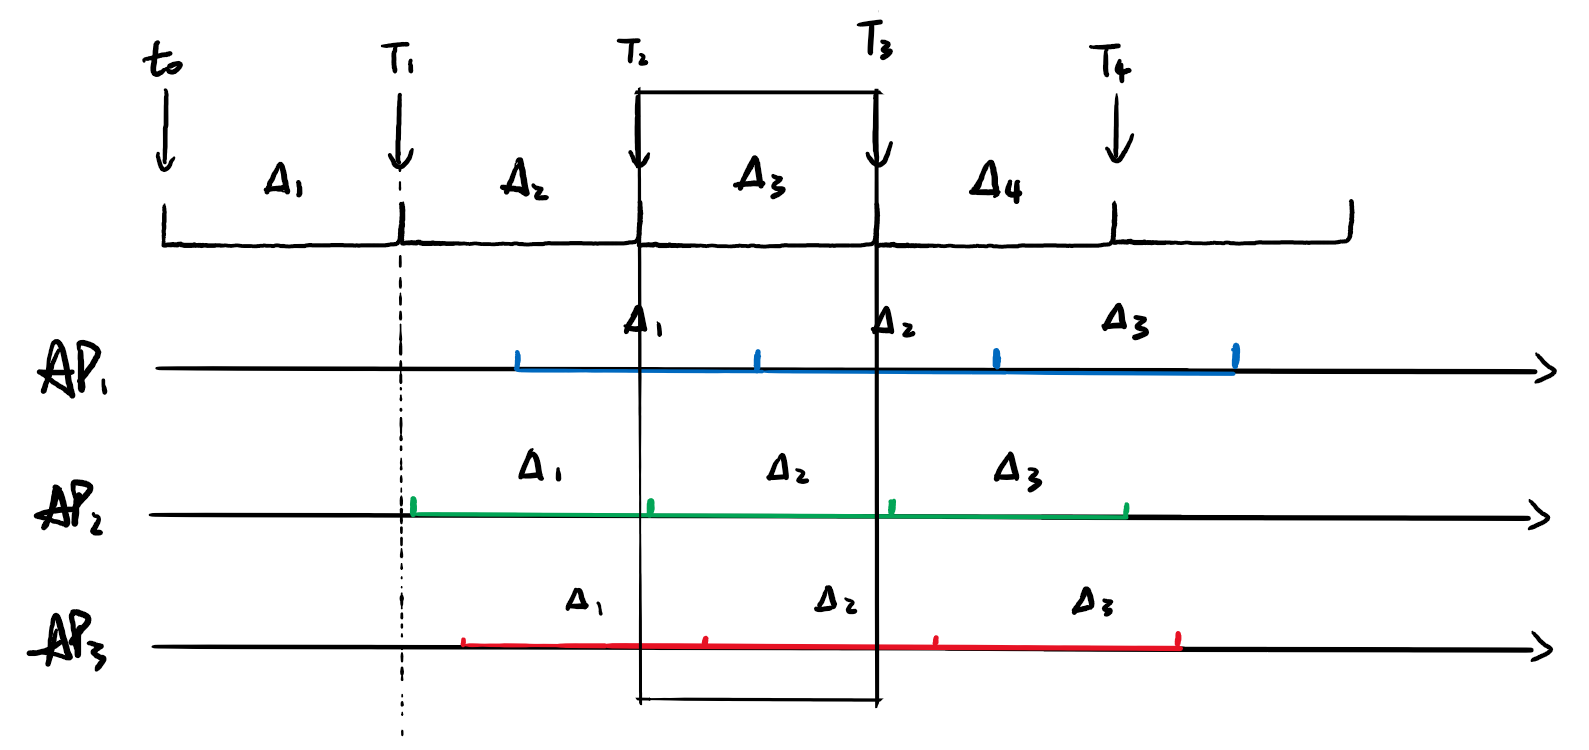
\includegraphics[width=0.45\textwidth]{broadcast-trans.png}
                \caption{Global Consensus and Transition with Delayed Action}
                \label{fig:br-trans}
            \end{figure}

            As the transition is initialized by \emph{dispatching decision} over arrival job in $t$-th timeslot on each AP, we give the definition for decision action space denotation here:
            \begin{definition}
                (Dispatching Action Space).
                The dispatching action space is applied job-wise for the arriving jobs in each timeslot and denoted as $a: (j, m) \in \jSpace \times \set{1,\dots,M}$, where $(j, m)$ denotes the action that $j$-type job should be uploaded to $m$-th ES.
            \end{definition}

            The dispatching policy $\vec{\Omega}(\Stat_i)$ is actually a compounded policy composed of dispatching policy of all AP nodes, based on two stage of broadcast with obsolete information $\Obsv_{i-1}$ and the updated information $\Obsv_{i}$. This compounded policy over action space is illustrated as following:
            \begin{definition}(Compounded Dispatching Policy).
                The compounded dispatching policy over $\Stat_{i}$ is defined as $\Policy(\Stat_{i})$ which is composed of the local policy $\Omega_k(\Stat_{i}), \forall k\in\apSet$ as:
                \begin{align}
                    \vec{\Omega}(\Stat_{i}) \define [\Omega_1(\Stat_{i}), \dots, \Omega_K(\Stat_{i})]
                \end{align}
                More specifically, $\Omega_k(\Stat_{i})$ is composed of two-stage policy with $\omega_k(\Obsv_{i-1})$ and $\omega_k(\Obsv_{i})$ as:
                \begin{align}
                    \Omega_k(\Stat_i) = 
                    \begin{cases}
                        \set{\omega^{(i-1)}_{k,m}(j)|\forall m\in\esSet}, & 0 \leq \Delta{t} < t^{(d)}_k
                        \\
                        \set{\omega^{(i)}_{k,m}(j)|\forall m\in\esSet}, & t^{(d)}_k \leq \Delta{t} \leq t_B
                    \end{cases}
                \end{align}
                where $t\in[t_{i-1}, t_{i}], \Delta{t} \define t - t_{i-1}$; $\omega^{(i)}_{k,m}$ denotes the dispatching policy that: based on global information $\Obsv_{i}$, the stochastic action on $k$-th node upload $j$-type job ($\forall j\in\jSpace$) to $m$-th ES.
            \end{definition}
        \end{subsection}

        \begin{subsection}{The Optimization Problem}
            The optimization target of our problem is to minimize the \emph{average response time} of all jobs, which is composed of uploading time from AP to ES, and waiting time on ES and service time on ES. According to \emph{Little's Law}, the average time over all the jobs is equally as number in system accumulation in each timeslot. The cost function is:
            \begin{align}
                g \bigg( \Stat_{i}, \Policy(\Stat_{i-1}) \bigg) \define \sum_{k\in\apSet} \Inorm{\vec{u}_{k}(i)} + \sum_{m\in\esSet} \norm{Q_m(i)},
            \end{align}
            where $\norm{Q_m(i)}$ denotes the number of jobs in queue $Q_m(i)$.
            Our distributed optimization problem definition is given as following:
            \begin{problem}
                (Distributed Cooperative Job Dispatching Problem).
                \begin{gather}
                    \min_{\Policy} \lim_{T \to \infty}
                        \mathbb{E}_{\Policy, \{A_k(t)|\forall k\in\apSet\}}
                            [\sum_{i=2}^{T} \gamma^{i-1} g(\Stat_{i}, \Policy(\Stat_{i-1}))|\Stat_1]
                \end{gather}
            \end{problem}

            According to \cite{sutton1998introduction}, the above problem could be solved by the following \emph{Bellman's equation}:
            \begin{align}
                V(\Stat_{i}) =& g(\Stat_i) + \gamma \min_{\Policy(\Stat_{i})} \sum_{\Stat_{i+1}} \Pr\{ \Stat_{i+1}|\Stat_{i}, \Policy(\Stat_{i}) \} V(\Stat_{i+1})
                \nonumber\\
                =& g(\Stat_{i}) + \gamma \min_{\Policy(\Stat_{i})} \sum_{\Stat_{i+1}} \Pr\{ \Stat_{i+1}|\Stat_{i}, \Policy(\Stat_{i}) \}
                    \nonumber\\
                    & \cdot [W^{(AP)}(\vec{u}_k(i+1)) + W^{(ES)}(\Obsv(i+1))],
            \end{align}
            where $W^{(AP)}(\cdot)$ and $W^{(ES)}(\cdot)$ denote the split value function over AP nodes and ES nodes respectively, which are denoted as:
            \begin{gather}
                W^{(AP)}(\set{\vec{u}_k(i)|k\in\apSet}) \define \mathbb{E}_{\Policy}[\sum_{n=0}^{\infty} \gamma^{n} \sum_{k\in\apSet}\Inorm{\vec{u}_k(i+n)}]
                \\
                W^{(ES)}(\Obsv(i)) \define \mathbb{E}_{\Policy}[\sum_{n=0}^{\infty} \gamma^{n} \sum_{m\in\esSet}|Q_m(i+n)|],
            \end{gather}
            where $\Inorm{\vec{u}_k(i)}$ denotes l1-norm of the vector, i.e. the sum-up of absolute value of each entry of vector; and $|Q_m(i)|$ denotes the cardinality of the set.

            Before diving into analysis on the transition function expression, we come up with some probability denotations. As we take the uploading process as \emph{black box}, the job-type information is unknown in uploading until the time when the jobs join the computation queue. We separate the probability expression of jobs arrival process for ES nodes into two parts as: arrival numbers distribution, and arrival job-types distribution.

            The arrival numbers distribution is composed of Bernoulli distribution in each timeslot, which from $k$-th AP to $m$-th ES under policy $\omega^{(i)}_{k,m}$ with PMF (probability mass function) expression as:
            \begin{align}
                p^{(\lambda,i)}_{k,m} \define \lambda_k \sum_{j\in\jSpace} p(j) \Pr\{\omega^{(i)}_{k,m}(j)\},
                % \nonumber\\
                % \Pr\{\text{one job from $k$-AP to $m$-ES under policy $\omega^{(i)}$}\}
            \end{align}
            and $p^{(\lambda,\Pi_k)}_{k,m}$ denotes the distribution under fixed policy $\Pi_{k}$ for $k$-th AP not with respect to system state.
            \\
            The job distribution on $m$-th ES under policy $\omega^{i}_{k,m}$ from $k$-th AP is denoted as:
            \begin{align}
                p^{(\theta, i)}_{k,m}(j) \define p(j) \Pr\{\omega^{(i)}_{k,m}(j)\}, \forall j\in\jSpace
            \end{align}
            where $\sum_{j\in\jSpace}\sum_{k\in\apSet}\sum_{m\in\esSet} p^{(\theta, i)}_{k,m}(j)=1, p^{(\theta, i)}_{k,m}(j) \geq 0$; and we have $p^{(\theta,Pi)}_{k,m}(j)$ denotes the process under policy $\Pi_k$ for $k$-th AP nodes not with respect to system states.

            Then we try to decouple the transition probability expression for AP nodes and ES nodes respectively as:
            \begin{align}
                & \Pr\{\Stat_{i+1}|\Stat_{i}, \Policy(\Stat_{i})\} 
                \nonumber\\
                =& \Pr\{\set{\vec{u}_k(i+1)|\forall k\in\apSet}, \set{Q_m(i+1)|\forall m\in\esSet}
                    \nonumber\\
                    &|\set{\vec{u}_k(i)|\forall k\in\apSet}, \set{Q_m(i)|\forall m\in\esSet}, \Policy(\Stat_{i})\}
                \nonumber\\
                =& \prod_{k\in\apSet} \Pr\{\vec{u}_k(i+1)|\Policy(\Stat_{i})\} \times
                    \nonumber\\
                    & \prod_{m\in\esSet} \Pr\{Q_m(i+1)|Q_m(i), \set{\vec{u}_k(i)|\forall k\in\apSet}, \Policy(\Stat_{i})\}
            \end{align}
            
            The first production part denotes the state transition for AP nodes whose distribution follows a Binomial distribution with the summed up i.i.d Bernoulli distribution. The state transition for $k$-th AP node is given as:
            \begin{align}
                \Pr\{\vec{u}_k=\vec{u}|\Policy(\Stat_i)\} \sim \prod_{m\in\esSet} Bin(t^{(u)}_{k,m}-1,p^{(\lambda, i)}_{k,m}),
                % \nonumber\\
                % =& \prod_{m\in\esSet}
                %     \begin{pmatrix}
                %         t^{(u)}_{k,m}-1 \\ u^{(m)}
                %     \end{pmatrix}
                %     (p^{(i)}_{k,m})^{u^{(m)}}
                %     (1-p^{(i)}_{k,m})^{T^{(prop)}_{k,m}-u^{(m)}-1}
            \end{align}
            where $Bin(n,p)$ denotes a Binomial distribution.
            \\
            The second part denotes the state transition for ES nodes. As the jobs to computing in this broadcast interval only contains the jobs in queue in last interval, the expression of $Q_m(i+1)$ could be:
            \begin{align}
                Q_m(i+1) = [\tilde{Q}_m(i), Y_0, Y_1, Y_2],
            \end{align}
            where:
            \begin{itemize}
                \item $\tilde{Q}_m(i)$ denotes the remaining part of $Q_m(i)$ after $t_B$ timeslots computing in $[t_{i}, t_{i+1}]$;
                \item $Y_0$ denotes the enqueued job set from last interval from unfinished uploading jobs in last interval as $\set{u_{k,m}(i)|\forall k\in\apSet}$, where $n^{(k)}_0 \define u_{k,m}(i)$, $|Y_0|=\sum_{k\in\apSet} u_{k,m}(i)$;
                \item $Y_1$ and $Y_2$ respectively denotes the enqueued job set uploaded by all AP nodes under policy $\omega_{k,m}^{i-1}$ and $\omega_{k,m}^{i}$, where $|Y_1|\define\sum_{k\in\apSet}N^{(k)}_1, |Y_2|\define\sum_{k\in\apSet}N^{(k)}_2$.
            \end{itemize}
            Then transition function for state transition for $m$-th ES node is given as:
            \begin{align}
                & \Pr\{Q_m(i+1)|Q_m(i), \set{\vec{u}_k(i)|\forall k\in\apSet}, \Policy(\Stat_i)\}
                \nonumber\\
                =& \Pr\{\tilde{Q}_m(i)|Q_m(i)\} \cdot \Pr\{Y_0, Y_1, Y_2|\set{\vec{u}_k(i)|\forall k\in\apSet}, \Policy(\Stat_i)\}
                \nonumber\\
                =& \prod_{k\in\apSet} [Bin(t^{(d)}_k, p^{(\lambda, i-1)}_{k,m}) \cdot \prod_{i=n}^{n^{(k)}_0 + N^{(k)}_1} p^{(\theta, i-1)}_{k,m}(j_n)]
                \nonumber\\
                & \times [Bin(t_B-t^{(d)}_k-t^{(u)}_{k,m}, p^{(\lambda, i)}_{k,m}) \cdot \prod_{i=1}^{N^{(k)}_2} p^{(\theta, i)}_{k,m}(j_n)]
                % \nonumber\\
                % =& \prod_{k\in\apSet} [\prod_{i=n}^{n^{(k)}_0 + N^{(k)}_1} p^{(i-1)}_{k,m}(j_n)
                %     \begin{pmatrix}
                %         t^{(d)}_k \\ N^{(k)}_1
                %     \end{pmatrix}
                %     (p^{(i-1)}_{k,m})^{N^{(k)}_1}
                %     \nonumber\\
                %     &(1-p^{(i-1)}_{k,m})^{t^{(d)}_k-N^{(k)}_1}] \cdot [\prod_{i=1}^{N^{(k)}_2} p^{i}_{k,m}(j_n)
                %     \begin{pmatrix}
                %         t_B-t^{(d)}_k-t^{(u)}_{k,m} \\ N^{(k)}_2
                %     \end{pmatrix}
                %     \nonumber\\
                %     &(p^{(i)}_{k,m})^{N^{(k)}_2} (1-p^{(i)}_{k,m})^{\tilde{N}^{(k)}_2}],
            \end{align}
            where $Bin(n,p)$ denotes the Binomial distribution.
        \end{subsection}
    \end{section}

    %============================= ALGORITHM ==============================%
    \begin{section}{LOW-COMPLEXITY SOLUTION}
        \label{sec:algorithm}
        As the formulated problem above is of infinite states and the action space would be exponentially expanded with respect to number AP and ES nodes, we could not use traditional \emph{policy iteration} or \emph{value iteration} algorithm \cite{sutton1998introduction} for unacceptable computational complexity.
        To alleviate curse of dimensionality, we take baseline dispatching policy to approximate the value function for each AP and ES nodes, and then carry out one-step iteration to obtain a better value function approximation.

        \begin{subsection}{Baseline Dispatching Policy}
            The baseline dispatching policy is adopted to obtain an approximation of value function. The policy on each AP nodes is randomized and time-invariant which is denoted as:
            \begin{align}
                \vec{\Pi} \define [\Pi_1, \Pi_2, \dots, \Pi_K],
            \end{align}
            where $\Pi_k = \set{\omega_{k,m}|\forall m\in\esSet}$, $\forall k\in\apSet$.

            The decoupled value functions for AP and ES nodes is obtained with an approximated form under the baseline policy.
            
            The approximated value function $\tilde{W}^{(AP)}$ for AP nodes is illustrated as:
            \begin{align}
                &\tilde{W}^{(AP)}(\set{\vec{u}_k(i+1)|k\in\apSet})
                \nonumber\\
                \define& \lim_{T\to\infty} \mathbb{E}_{\vec{\Pi}}[\sum_{n=0}^{T} \gamma^{n} \sum_{k\in\apSet} \Inorm{\vec{u}_k(i+n+1)}]
                \nonumber\\
                =& \lim_{T\to\infty} \sum_{n=0}^{T} \gamma^{n} \mathbb{E}_{\vec{\Pi}}[\sum_{k\in\apSet} \Inorm{\vec{u}_k}]
                \nonumber\\
                =& \frac{1}{1-\gamma} \sum_{k\in\apSet} \mathbb{E}_{\Pi_k}[\Inorm{\vec{u}_k}],
            \end{align}
            where the expectation of $\Inorm{\vec{u}_k}$ under the policy $\Pi_k$ is calculated with a Binomial distribution as:
            \begin{align}
                \mathbb{E}_{\Pi_k}[\Inorm{\vec{u}_k}] =& t^{(u)}_{k,m} \times p^{(\lambda, \Pi_k)}_{k,m}
                \nonumber\\
                =& \lambda_k t^{(u)}_{k,m} \sum_{j\in\jSpace} \Pr\{\omega_{k,m}(j)\},
            \end{align}
            which is actually a constant under fixed policy $\Pi_k$.
            
            The approximated value function $\tilde{W}^{(ES)}(\Obsv(i))$ for ES nodes is affected with both arrival process under dispatching policy and last queue state, and we reduce the states expression by averaging the uploading process. For convenience, we have $\Stat^{(AP)}(i) \define \set{\vec{u}_k(i)|\forall k\in\apSet}$ and $\Stat^{(ES)}(i) \define \set{Q_m(i)|\forall m\in\esSet}$.
            The probability expression for partial ES value function optimization in Bellman's Equation is given as:
            \begin{align}
                \min_{\Policy(\Stat_i)}& \sum_{\Stat_{i+1}} \Pr\{\Stat_{i+1}|\Stat_{i}, \Policy(\Stat_i)\} \cdot \tilde{W}^{(ES)}(\Obsv(i+1))
                \nonumber\\
                \leadto \min_{\Policy(\Stat_i)}& \sum_{\Stat^{(ES)}(i)} \Pr\{\Stat^{(ES)}(i+1)|\Stat^{(ES)}(i),\Stat^{(AP)}(i), \Policy(\Stat_i)\}
                    \nonumber\\
                    & \times \sum_{\Stat^{(AP)}(i)} \Pr\{\Stat^{(AP)}(i+1)|\Policy(\Stat_i)\} \cdot \tilde{W}^{(ES)}(\Obsv(i+1))
                \nonumber\\
                \leadto \min_{\Policy(\Stat_i)}& \sum_{\Stat^{(ES)}(i)} \Pr\{\Stat^{(ES)}(i+1)|\Stat^{(ES)}(i),\Stat^{(AP)}(i), \Policy(\Stat_i)\}
                    \nonumber\\
                    & \times \sum_{m\in\esSet} \mathbb{E}_{\Stat^{(AP)}(t+1)|\Policy(\Stat_t)}[\tilde{W}^{(ES)}_m(\Obsv(i+1)],
            \end{align}
            let $\tilde{V}(Q_m(i+1)) \define \mathbb{E}_{\Stat^{(AP)}(t+1)|\Policy(\Stat_t)}[\tilde{W}^{(ES)}_m(\Obsv(i+1)]$ denotes the averaged value function for $m$-th ES nodes, which implies that the arrival process in approximated value function is average with the process under policy $\Policy(\Stat_i)$.

            Furthermore, the approximated value function could be rewrite with reduced states for stationary FCFS process as $\tilde{V}(\tilde{Q}_m(i+1))$, where $\tilde{Q}_m(i+1) \define [N_m(i+1), r_m(i+1)]$, $N_m(i+1)$ denotes the number of jobs in $m$-th queue and $r_m(i+1)$ denotes the remaining time of last unfinished job. Thus the approximated value function for $m$-th ES node is denoted as:
            \begin{align}
                \tilde{V}(\tilde{Q}_m(i+1)) =& \lim_{T\to\infty} \mathbb{E}_{\vec{\Pi}} [\sum_{n=0}^{T} \gamma^{n} N_m(i+1)]
                \nonumber\\
                =& \vec{u}'_i [\lim_{T\to\infty} \sum_{n=0}^{T} (\gamma \mat{P}_m)^{n}] \vec{g}_q
                \nonumber\\
                =& \vec{u}'_i (\mat{I} - \gamma \mat{P}_m)^{-1} \vec{g}_q,
            \end{align}
            where $\vec{\mu}'_i$ denotes the transpose of $\vec{\mu}_i$, and $\vec{\mu}_i = [0,\dots,0,1,\dots]$ with only $i$-th element as $1$; the $i$-th element of $\vec{g}_q$ denotes the cost of server as $N_m(i)$ for $i$-th stage; $\mat{P}_m$ denotes the transition matrix under the policy $\vec{\Pi}$ which is composed of the following transition function ($\forall \tilde{Q}_m(i),\tilde{Q}_m(i+1)$) as:
            \begin{align}
                & \Pr\{\tilde{Q}_m(i+1)|\tilde{Q}_m(i),\vec{\Pi}\}
                \nonumber\\
                =& \Pr\{\begin{pmatrix}
                    N_m(i+1) \\ r_m(i+1)
                \end{pmatrix}|\begin{pmatrix}
                    \tilde{N}_m(i+1) \\ r_m(i)
                \end{pmatrix}\}
                \nonumber\\
                =& \prod_{k\in\apSet} \Pr\{\tilde{N}^{(k)}_m(i+1)\} \times \prod_{n=0}^{\tilde{N}^{(k)}_m(i+1)} p^{(\theta,\Pi_k)}_{k,m}(j_{k,n})
                \nonumber\\
                &\times I[\sum_{j_{k,n}} f(j_{k,n})^{(m)} = r_m(i+1)+t_B-r_m(i)]
            \end{align}
            where $f:\jSpace \to \domZ^M$ is the mapping function from job-type index to computing time on all servers and $\tilde{N}^{(k)}_m(i+1)$ denotes:
            \begin{gather}
                \tilde{N}^{(k)}_m(i+1) = t^{(u)}_{k,m} + Bin(t_B-t^{(u)}_{k,m}, p^{(\lambda, \Pi_k)}_{k,m}), \forall k\in\apSet
            \end{gather}
        \end{subsection}

        \begin{subsection}{The Distributed Algorithm}
            Then we introduce the one-step iteration algorithm in this section:
            % [\IF, \ENDIF], [\FOR, \TO, \ENDFOR], [\WHILE, \ENDWHILE], \STATE, \AND, \TRUE
            \begin{algorithm}[H]
                \caption{Distributed Algorithm for $k$-th AP}
                \begin{algorithmic}
                    \WHILE{\TRUE}
                        \STATE (in progress...)
                        % \FOR{$k \in \mathcal{K}$}
                        %     \STATE fix policy $\vec{\Omega}^{(k)}(t) \forall k' \neq k$
                        % \ENDFOR
                    \ENDWHILE
                \end{algorithmic}
            \end{algorithm}
        \end{subsection}
        
    \end{section}

    %============================ EVALUATION ==============================%
    \begin{section}{EVALUATION}
        \label{sec:evaluation}
        (in progress)
    \end{section}

    %============================= CONCLUSION =============================%
    \begin{section}{CONCLUTION}
        \label{sec:conclusion}
        The future work to mention:
        \begin{itemize}
            \item joint scheduling optimization
            \item non-aligned broadcast
            \item broadcast failure
            \item randomized broadcast delay
        \end{itemize}
    \end{section}

    %============================== REFERENCE =============================%
    \bibliographystyle{IEEEtran}
    \bibliography{main.bib,journal-ref.bib}
\end{document}